\begin{figure*}[!ht]
 \centering
 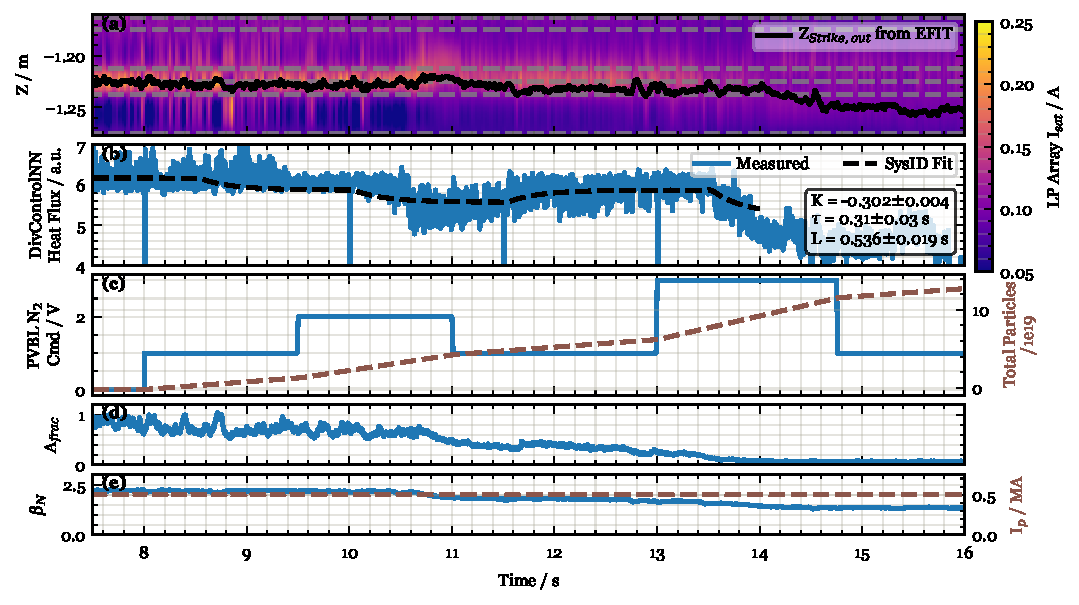
\includegraphics[width=\textwidth]{figures/DetCtrl_2D_35854.pdf}
 \caption{System identification shot \#35854.
(a) Shows the measured ion saturation current by realtime Langmuir Probe array at locations marked by grey dashed lines.
The data has been interpolated spatially using cubic spline interpolation.
The black curve shows the post-shot calculated strike point position on outer divertor using EFIT.
(b) Shows the heat flux at outer divertor calculated by DivControlNN.
The dashed black line shows the system identification fit on this data.
(c) Left axis: Shows the N$_2$ gas command steps sent for system identification.
Right axis: Shows the cummulative N$_2$ gas particles injected into the vessel.
(d) Shows the \Afrac calculated from peak value among the Langmuir probe array.
(e) Left axis: Shows $\beta_n$.
Right axis: Shows the plasma current (I$_p$).}
\label{fig:sysid_sm}
\end{figure*}